\section{Visão Geral da Implementação}\label{4-grasews-visao-geral-implementacao}

O módulo de \textit{front-end} foi desenvolvido seguindo a arquitetura MVC provido pelo \textit{ASP.NET MVC}~\cite{MICROSOFT-2019-ASP-NET-MVC}. Neste módulo, a biblioteca \textit{jQuery}~\cite{JQUERY-2019} foi intensivamente utilizada em conjunto com a linguagem \textit{JavaScript} para o desenvolvimento de funcionalidades do lado cliente para o módulo de \textit{front-end}. Adicionalmente, para a formatação da interface gráfica de usuário de Grasews, as linguagens HTML5 e CSS3 foram utilizadas, ambas suportadas por \textit{templates} providos por \textit{Admin LTE}~\cite{ADMIN-LTE-2019}, por funcionalidades providas por \textit{Bootstrap}~\cite{BOOTSTRAP-2019} e por ícones providos por \textit{Font-Awesome}~\cite{FONT-AWESOME-2019}.

O formato padrão de comunicação entre o \textit{front-end} e o \textit{back-end} é o formato JSON~\cite{JSON-2019}. Neste sentido, todas as mensagens utilizadas nas interações entre os a interface de usuário e a API da aplicação utilizam objetos JSON. Adicionalmente, o formato JSON é utilizado na criação dos grafos da ferramenta, provido pela biblioteca \textit{Cytoscape.js}\cite{CYTOSCAPE-2015}.

As principais linguagens de programação utilizadas no desenvolvimento da ferramenta Grasews foi o linguagem C\#, do \textit{framework} .NET~\cite{MICROSOFT-2019-NET-FRAMEWORK}. C\# possibilitou o desenvolvimento de funcionalidades do lado servidor providas pelos módulos de \textit{back-end} da aplicação. A API da aplicação foi desenvolvida como serviços web RESTful, suportados pelo \textit{ASP.NET Web API}~\cite{MICROSOFT-2019-WEB-API}. Adicionalmente, a utilização do ORM \textit{.NET Entity Framework}~\cite{MICROSOFT-2019-Entity-Framework} possibilitou uma mais fácil implementação do mapeamento de classes .NET para tabelas do banco de dados, bem como na criação da estrutura do banco de dados (\textit{migrations}) e na persistência de dados da aplicação no \textit{Postgres}~\cite{POSTGRES-2019}.

Um conjunto de ferramentas foi utilizado no desenvolvimento de Grasews. A seguir, são listadas as principais ferramentas que deram suporte ao desenvolvimento de Grasews.

\begin{enumerate}

  \item \textbf{Microsoft Visual Studio 2017 e 2019}
  
  \textit{Microsoft Visual Studio} é um ambiente (IDE) de desenvolvimento para linguagens de programação do \textit{framework} .NET, entre outras. \textit{Visual Studio} provê fácil integração com \textit{Microsoft Azure} e com \textit{Microsoft Azure DevOps}, para publicação de aplicações e controle de versão do código-fonte, respectivamente. Todos os módulos de Grasews foram desenvolvidos utilizando o \textit{Visual Studio}.
  
  %Para mais informações, consulte \href{https://visualstudio.microsoft.com/}{https://visualstudio.microsoft.com/}
  
  \item \textbf{pgAdmin}
  
 \textit{pgAdmin}~\cite{PGADMIN-2019} é a plataforma de administração e desenvolvimento mais popular e com mais recursos para o banco de dados \textit{PostgreSQL}. Assim como \textit{PostgreSQL}, \textit{pgAdmin} é desenvolvido com o códio aberto. Durante o desenvolvimento de Grasews, a fim de validar os
  
  %Para mais informações, consulte \href{https://www.pgadmin.org/}{https://www.pgadmin.org/}
  
  \item \textbf{Postman}
  
  \textit{Postman}~\cite{POSTMAN-2019} é uma plataforma de colaboração para o desenvolvimento de APIs. Os recursos do \textit{Postman} simplificam cada etapa da criação de uma API e agilizam a colaboração para que você possa criar APIs mais rapidamente. Utilizamos \textit{Postman} para validar as funcionalidades disponíveis em \texttt{Grasews.API}, bem como para agilizar o uso da ferramenta de uma perspectiva do desenvolvimento. Uma coleção de requisições para \texttt{Grasews.API} foi criada e salva \textit{Postman} Com isso, podemos validar tanto os endereços dos \textit{endpoints}, quanto os parâmetros de entrada e as respostas dos \textit{endpoints}.
  
  %Para mais informações, consulte \href{https://www.getpostman.com/}{https://www.getpostman.com/}
  
  \item \textbf{Microsoft Azure Hosting}
  
  \textit{Microsoft Azure}~\cite{MICROSOFT-2019-AZURE} é um serviço de computação em nuvem criado por \textit{Microsoft} para criar, testar, implantar e gerenciar aplicativos e serviços por meio de data centers gerenciados por \textit{Microsoft}. Utilizamos \textit{Microsoft Azure} para hospedar tanto \texttt{Grasews.Web} quanto \texttt{Grasews.API}. O endereço web de \texttt{Grasews.Web} é  \href{https://grasewsweb.azurewebsites.net/}{https://grasewsweb.azurewebsites.net/} e de \texttt{Grasews.API} é  \href{https://grasewsapi.azurewebsites.net/}{https://grasewsapi.azurewebsites.net/}.
  
  %Para mais informações, consulte \href{https://azure.microsoft.com/}{https://azure.microsoft.com/}
  
  \item \textbf{Microsoft Azure DevOps}
  
  \textit{Microsoft Azure DevOps}~\cite{MICROSOFT-2019-DEVOPS} é um repositório de código-fonte oferecido por \textit{Microsoft}. Por meio de \textit{Microsoft Azure DevOps}, desenvolvedores podem versionar o código-fonte, bem como controlar as entregas e automatizar tarefas como compilações e publicações de aplicações. Todo o código-fonte de Grasews está controlado por meio de \textit{Microsoft Azure DevOps}. O endereço web do repositório é \href{https://dev.azure.com/matheuscalache/Grasews}{https://dev.azure.com/matheuscalache/Grasews}.
  
  %Para mais informações, consulte \href{https://azure.microsoft.com/en-us/services/devops/}{https://azure.microsoft.com/en-us/services/devops/}
  
\end{enumerate}

A \figurename~\ref{fig:grasews-technology-stack} apresenta a pilha de tecnologias utilizada na arquitetura de desenvolvimento do Grasews. No topo, encontramos as tecnologias utilizadas para o desenvolvimento da camada de \textit{front-end} de Grasews, i.e., a interface gráfica de usuário. Nesta camada, à esquerda encontramos as principais tecnologias utilizadas do \textit{framework} .NET. Ao centro da camada de \textit{front-end}, encontramos as principais tecnologias e bibliotecas utilizadas para o desenvolvimento com base na linguagem \textit{JavaScript}. Por fim, acima das bibliotecas \textit{JavaScript}, encontramos as principais tecnologias e bibliotecas utilizadas para formatação e apresentação de páginas web (HTML e CSS). Abaixo da camada de \textit{front-end}, são representadas as principais tecnologias utilizadas para o desenvolvimento da camada de \textit{back-end}. Nesta camada utilizamos exclusivamente tecnologias do \textit{framework} .NET. A próxima camada é a camada de persistência de dados. Nesta camada, encontramos o uso do banco de dados Postgres. Por fim, a camada na base da figura apresenta a plataforma de hospedagem e controle de código-fonte, provida pela solução em nuvem \textit{Microsoft Azure}.

O Apêndice \ref{apendice-tecnologias-grasews} apresenta uma visão geral das principais tecnologias e bibliotecas de desenvolvimento utilizadas na implementação de Grasews.

\begin{landscape}
    \begin{figure}[h]
        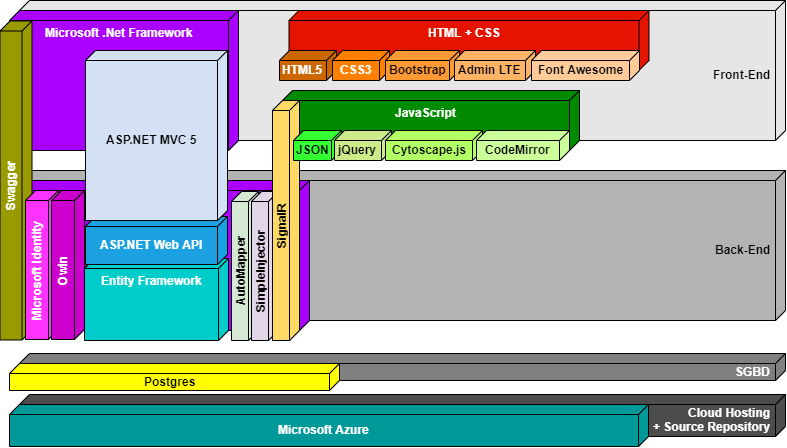
\includegraphics[scale=0.7]{4-grasews/imagens/grasews-technology-stack.png}
        \centering
        \caption[Pilha de tecnologias envolvidas no desenvolvimento do Grasews]{\textbf{Pilha de tecnologias envolvidas no desenvolvimento do Grasews.}}
        \label{fig:grasews-technology-stack}
    \end{figure}
\end{landscape}